% Template for ICIP-2019 paper; to be used with:
%          spconf.sty  - ICASSP/ICIP LaTeX style file, and
%          IEEEbib.bst - IEEE bibliography style file.
% --------------------------------------------------------------------------
\documentclass{article}
\usepackage{spconf,amsmath,graphicx, url}
\usepackage{enumitem, booktabs, multirow}
\usepackage[table,xcdraw]{xcolor}
\usepackage{arydshln}

\usepackage{caption}
\captionsetup[table]{justification=centerlast,
                     labelsep=newline,
                     font=sf,
                     textfont=footnotesize}
\captionsetup[figure]{justification=centerlast,
                     font=sf,
                     textfont=footnotesize}

\renewcommand\thetable{\Roman{table}} %Make the table's captions Roman numerals
% \setlength{\parskip}{0.1em}

%\parskip 0.2in %Separation between paragraphs
% Example definitions.
% --------------------
\def\x{{\mathbf x}}
\def\L{{\cal L}}

% Title.
% ------
\title{MRI-SPECT Image Fusion using Wavelet Transforms and Particle Swarm Optimization of Image Fusion Performance Metric}
%
% Single address.
% ---------------
%\name{Author(s) Name(s)\thanks{Thanks to XYZ agency for funding.}}
%\address{Author Affiliation(s)}
%https://de.overleaf.com/project/5d8d41d85f86a90001d55d6d
% For example:
% ------------
%\address{School\\
%	Department\\
%	Address}
%
% Two addresses (uncomment and modify for two-address case).
% ----------------------------------------------------------
\twoauthors
  {Gomez Gonzalez, Juan M. \textsuperscript{1}; Hoyos Velasquez, Natalia \textsuperscript{1}; Zaki, Shadi \textsuperscript{1}; Woidelko, Mirco F. \textsuperscript{2} \sthanks{The author performed the work while at University of Waterloo}}
	{\small \textsuperscript{1} Dept. of Electrical and Computer Engineering, University of Waterloo, CA. \\
	\small \textsuperscript{2} Dept. of Mechanics and Ocean Engineering, Hamburg University of Technology, DE.}
  {}
	{}

\begin{document}
%\ninept
%
\maketitle

\begin{abstract}
\ninept
\textbf{
Despite the effort in image fusion research, there does not yet exist a golden rule to fuse images and ensure proper information retention. For medical image fusion, it is important that the fused image conserves the relevant information of the source images.
Thus, this paper proposes a new fusion rule applied on MRI and SPECT images using particle swarm optimization and image fusion performance metric (IFPM) to improve the information density of the fused image with respect to the original images for better medical diagnosis. The results obtained are compared using entropy (EN) and mutual information (MI).
The proposed fusion model shows higher values for IFPM as well as MI. From the results, it can be inferred that the proposed method improved the information content, which may lead to better decision for diagnosis.} 
\end{abstract}
%
\begin{keywords}
\ninept
Discrete Wavelet Transform (DWT), entropy, image fusion evaluation, Image Fusion Performance Metric (IFPM), mutual information, Multiwavelet Transform (MWT), Particle Swarm Optimization (PSO)
\end{keywords} 
%
\section{Introduction}
\label{sec:intro}
Image fusion is an important topic in medical image processing. It is an attempt to bundle all information of multi-modal images into a single image. This compact representation of information could facilitate the work of radiologists and allow for more informed decisions.  
During the past decades, different image fusion rules for wavelet transform methods have been developed. According to \cite{S.Polinati.2019}, the most recent rules are principal component analysis, maximum rule, (weighted) averaging, and directive contrasts.
%Also Wiener Filter \cite{Goel.2017} or visibility based image fusion \cite{M.Haribabu.2017} have been proposed to improve the information content. 
Others, like \cite{Wang2004}, use two different rules for lower and higher frequency sub-bands and optimize using mutual-information.
%Besides from the deterministic fusion rules, adapting rules, e.g. genetic grey-wolf optimization algorithm by \cite{Daniel.2018} have been proposed in the past years.
%However, despite the many different attempts there does not yet exist a optimal fusion rule. There are two reasons for this. The first reason is the requirement for versatility in the fusion rule to accommodate the different modalities. Second, the existing quality metrics have a limited validity and do not reflect the human perception metric. According to \cite{S.Polinati.2019}, common quality metrics are entropy (EN), standard deviation (SD), mutual information (MI), and structural similarity index measure (SSIM), peak to noise ratio (PSNR).
Similarly, some fusion optimization algorithms have incorporated quality metrics as utility functions. For example, \cite{Ravichandran.2017} proposed a method using particle swarm and entropy for the optimal fusion in discrete wavelet transform for CT and MRI images among others. The work by \cite{Dou.2019} uses a genetic algorithm and image quality index, a metric introduced in \cite{ZhouWang.2002}, to enhance performance of fusion together with wavelet transforms for different fields, in which image fusion is used. 
Thus, this paper extends on the idea of \cite{Ravichandran.2017} to use particle swarm optimization (PSO) to optimize the fusion rule.
Instead of using entropy as a utility function, image fusion performance measure (IFPM) is employed. IFPM allows to relate the information content of the fused image to the information content of the original images and was first proposed by \cite{ifpm}. Furthermore, the proposed fusion rule optimization is tested using discrete wavelet transform as well as multiwavelet transform on MRI and SPECT images taken from \cite{HarvardBrain}.
This paper is organized as follows: In section two, the wavelet transforms, IFPM, and PSO are introduced. Section three explains the proposed technique. Afterwards, the results are presented and discussed in section four. Finally, section five summarizes the findings and concludes the paper.

\section{Technical Background}
\subsection{Discrete and Multiwavelet Transform}
\label{subsec:DWT_MWT}
Wavelet transforms allow the decomposition of an image in terms of different locally oscillating wavelets that preserve its information.
%and is based on the idea of replacing the sinusoidal functions of the Fourier transform, which oscillate infinitely, with wavelets that consist of locally oscillating basis functions with an amplitude that begins at zero, increases, and then fades back to zero. 
Discrete Wavelet Transform (DWT) uses both shifting and scaling operations to obtain information related to the time and directional frequency, resulting in an image divided into four sub-bands or sub-images: low-low (LL), low-high (LH), high-low (HL), and high-high (HH). The LL sub-band can be considered as a smoothed as well as a sub-sampled version of the original image that contains the average information, whereas the other sub-bands contain details of horizontal, vertical, and diagonal directional information \cite{M.Haribabu.2017, Pajares.Delacruz.2004}.

In contrast, Multiwavelet Transform (MWT) uses multiple scaling and wavelet functions, allowing it to simultaneously possess properties like symmetry, orthogonality, and short support. Authors in \cite{Geronimo.1994} derived the Geronimo-Hardin-Massopust (GHM) construction and demonstrated which properties the parameters of the scaling and wavelet functions must fulfill to satisfy these conditions.

\subsubsection{Wavelet Transforms in Image Fusion}
For image fusion, the wavelet coefficients are obtained for different aligned and annotated images.
The coefficient pairs of corresponding resolution levels, frequencies, and representations are merged together with the guidance of a fusion rule. Fusion rules may depend on the application, and can either be applied to all the sub-bands equally or be frequency selective. Some of the rules are straightforward, like selecting the minimum, maximum, or mean values of the transform coefficients \cite{Pajares.Delacruz.2004, Chiorean.Vaida.2009}. Others, like \cite{Wang2004}, use different rules for lower and higher frequency sub-bands. In this case, the average of the wavelet coefficients is taken as a fusion rule for lower frequency sub-bands, since low frequencies in images represent their rough features. In higher frequencies, a pattern contrast-based measure is employed for pixel selection.

\subsection{Image Fusion Performance Metric}
\label{subsection: IFPM}
The IFPM is a global measure proposed by \cite{ifpm}. It attempts to objectively evaluate, based on information theory principles, the performance of image fusion schemes. It utilizes mutual information and mutual conditional information to quantify the amount of information that has been transferred from $N$ source images to one final fused image. For a set of source images $X_1, X_2, ... , X_n$, and a fused output image $Y$, IFPM is defined by Eq. \ref{eq:IFPM} \cite{ifpm}.

\begin{gather}\label{eq:IFPM}
% \ninept
IFPM = \frac{I(X_1,Y) + \sum_{i=2}^{N} I(X_i,Y|X_{i-1},...,X_1)}{H(X_1,X_2,...,X_n)}
\end{gather}

In this equation, $I(X_1,Y)$ represents the mutual information between the first source image $X_1$ and the final fused image $Y$.
$I(X_i,Y|X_{i-1},...,X_1)$ represents the conditional mutual information between source image $X_i$ and fused image $Y$, given all previously considered source images $X_{i-1},...,X_1$. Lastly, $H(X_1,X_2,...,X_n)$ represents the joint entropy of all source images. An IFPM value of $0$ indicates the absence of shared information among the source images and the fused result. If all the information in the source images is effectively transferred to the fused image, perfect fusion, the IFPM value becomes $1$ \cite{ifpm}.

There are two main features of IFPM that make it more appropriate for image fusion evaluation than other metrics. One of the objectives of any image fusion process is to incorporate multi-modal images in a compact manner while maximizing the amount of retained information. Moreover, medical images used for fusion are highly correlated due to being an image of the same physiological part through different imagining techniques.This results in a high information content overlap among the source images. IFPM, unlike other metrics, considers overlapping information only once through the conditional mutual information terms \cite{ifpm}. Another desirable feature of IFPM is that it is bounded between $0$ and $1$ making it easier to compare between different image fusion algorithms \cite{ifpm}. 

\subsection{Particle Swarm Optimization}
Particle Swarm Optimization (PSO) is a type of optimization in which multiple "particles" try to find the optimal solution similar to the behavior of a flock of birds \cite{Shi.Eberhart.1998}. The basic idea of this algorithm came from the study and simulation of social behavior by \cite{Kennedy.Eberhart.1995} in 1995 and was further developed by \cite{Shi.Eberhart.1998} in 1998 leading to what now is considered Swarm Theory.

The algorithm is initialized with a group of random solutions (akin to what can be seen in Genetic Algorithms), with the added benefit of also having a random number assigned to their velocities. The particles then try "flying" through the problem space from a random position and move towards the currently best-known solution. During this flyover, particles keep trying to find a more optimal solution in the problem space to replace this best-known solution iteratively \cite{Eberhart.Shi.2001}. The main advantage of PSO is that it has no need for the gradient of the problem, making it suitable for problems that have gradients too complex to derive \cite{Eberhart.Shi.2001}. At the same time, PSO's main disadvantage is that it requires fine-tuning of parameters that define the particles' velocities in order to prevent falling in a local optimum or "flying over" the optimal solution \cite{Eberhart.Shi.2001}.

% \section{Existing Fusion Rules}

% \subsection{Particle Swarm Optimization}
% \label{sec:eval}

% \section{Wavelet Transforms}
% \label{sec:WaveTrans}

% \subsection{Discrete Wavelet Transform}
% \label{subsec:DWT}
% The discrete wavelet transform (DWT) is a technique to decompose an image in terms of different wavelets that preserve the image information. Therefore, a basic wavelet, time limited, locally oscillating basis functions, is shifted or stretched to match the image information. Thereby, the DWT has a higher resolution in time domain and can present signals better than a Fourier Transform. However, the discrete nature causes that scaling of coefficients can results in aliasing after inverse transform. Similarly, it is sensitive to shifts and might cause ringing after the inverse transform. Moreover, positive and negative frequencies are not differentiated, which causes loss of information about directionality. Yet, for image fusion has been intensively researched in the past decades and optimized. Thus, new methods must benchmark oneself against the DWT with regard to computation and improvement in the information content of the fused image. 
% \subsection{Multiwavelet Transform}
% \label{subsec:MWT}


% \subsection{Dual-Tree Complex Wavelet Transform}
% \label{subsec:DtCWT}
% The dual-tree complex wavelet (DTCWT) is a method to determine real and imaginary coefficients of the wavelet transform. Therefore, two interlaced filter banks of DWT are used. One filter bank determines the real and the other bank the complex coefficient. Due to its approximate analytical form, DTCWT is almost shift-invariant, directional selective. Also scaling of the coefficients does not produce aliasing after the inverse-transform. However, the computation cost for this transform is also higher. Therefore, it is of interest if the improvements in the fused image justify the additional computational effort.

% \section{Evaluation of Image Fusion}
% \label{sec:eval}
% There exist a variety of methods to evaluate the performance of image fusion algorithms. The strictest, but also most subjective, performance measure, the human eye perception of the image. According to, the methods that are said to best match the impression of the human eye are:. Hence, these methods are used for evaluation of the information content of the fused image. Another measure is the computational cost and time to fuse the images. In today's spare server capacities at hospitals, it is also important to use the resources as efficient as possible. Furthermore, medical support is extended to rural areas with limited resources. Doctors increasingly use small portable tools to serve the patients needs, which have a limited computation power. Therefore, the respective computation time and power needed are also considered for the overall performance measure of an image fusion method.

% \subsection{Mean}
% \subsection{Entropy}
% \subsection{}

\section{Methods}
\label{sec: method}
This paper proposes an MRI-SPECT image fusion model and compares its performance with two other fusion rules: average rule and the technique developed by \cite{Wang2004}. The comparison is performed by first measuring and then contrasting the values obtained for IFPM, entropy (EN), and mutual information (MI) of the fused images. The proposed MRI-SPECT image fusion rule was performed using DWT and MWT and is based on an optimization of the acquired IFPM values through PSO. Fig. \ref{framework} shows the flow chart of the proposed image fusion model when applied to MWT. The following subsections describe the image fusion model in detail.

% This paper will compare the proposed fusion rule with images computed using the mean and the method developed by \cite{Wang2004}, applied on DWT and MWT.

\begin{figure*}[tb]
    \centering
    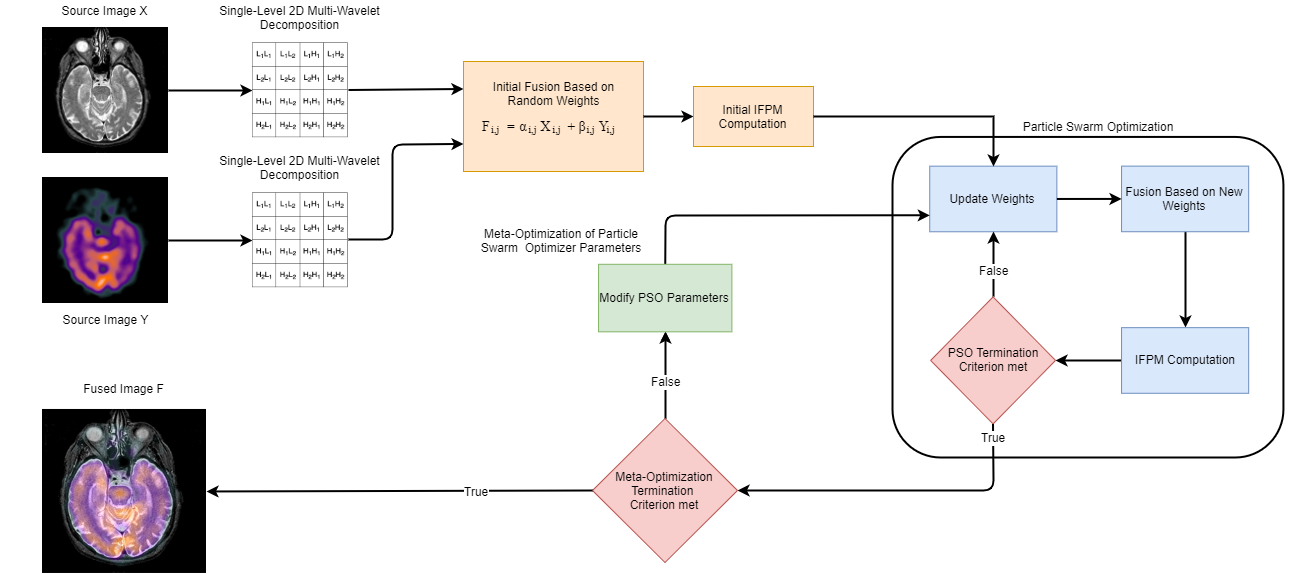
\includegraphics[height=8cm]{Img/Methodology.png}
    \caption{Flow Chart for the Proposed MRI-SPECT Image Fusion Model. Source images taken from \cite{HarvardBrain}.}
    \label{framework}
\end{figure*}
    
\subsection{Wavelet Transform Decomposition}
The first stage in the proposed MRI-SPECT image fusion model is the decomposition of the source images into their respective frequency sub-bands using the wavelet transforms. For the present experiment, DWT and MWT were independently used for decomposition.

\subsubsection{Discrete Wavelet Transform Decomposition}
The discrete wavelet decomposition used in this paper is a single level decomposition using the Daubechies 2 wavelet, used to obtain the 4 expected sub-bands for this level of decomposition (LL, LH, HL, HH) \cite{Pajares.Delacruz.2004}.

\subsubsection{Multiwavelet Transform Decomposition}
The multiwavelet decomposition employed in this paper is single-level and two-dimensional, meaning that each source image is decomposed into $16$ sub-bands as a result of two-dimensional filtering and based on two sets of high/low pass coefficients \cite{Wang2004}. Additionally, the implementation of the GHM multi-scaling construction decomposition by \cite{AlJewad.2006} was used in the present work for forward and inverse image transforms.

\subsection{Initial Fusion of Decomposed Sub-Bands and IFPM Evaluation}
The second stage in the proposed image fusion model is the initial fusion of the wavelet-decomposed sub-bands and the initial IFPM evaluation. The initial fusion process is modelled such that each sub-band of the fused result is computed as a weighted sum of the respective wavelet decomposition sub-bands of the source images. More formally, a fused sub-band, $F_{i,j}$, is computed using Eq. \ref{eq:5}.
\begin{gather}\label{eq:5}
F_{i,j} = \alpha_{i,j}X_{i,j} + \beta_{i,j}Y_{i,j}
\end{gather}
where $X_{i,j}$ and $Y_{i,j}$ are the source image sub-bands at position $(i,j)$, and $\alpha_{i,j}$ and $\beta_{i,j}$ are the weights assigned to $X$ and $Y$ at position $(i,j)$ respectively. In this step, the weights are randomly sampled from a uniform distribution to produce an initial fused image.

To reduce the complexity of the MWT model, the weight of the frequency sub-bands LL, LH, HL, and HH are shared across different channels, resulting in one weight for each individual frequency sub-band. This process yields a total of $8$ adjustable weights: $4$ for image $X$ and $4$ for image $Y$. Finally, an initial IFPM value is computed based on the resulting fused image.

\subsection{Particle Swarm Optimization of IFPM}
The next stage in the proposed fusion rule algorithm is the optimization of IFPM using PSO. Since IFPM provides an objective representation of the percentage of information that is transferred from the source images \cite{ifpm}, PSO should update weights in the direction of maximum information retention seeking an IFPM value that is as close to $1$ as possible.

The image fusion process as well as the IFPM evaluation is integrated within the actual PSO implementation, allowing the model to iteratively update the sub-band weights, perform fusions by adopting the new weights, and reevaluate an IFPM value based on the obtained fused result. Particularly, the PSO implementation used here is based on the one outlined in \cite{Zhang.Wang.Ji.2015}, with the termination criterion being $10$ iterations and the number of particles, $S$, being $25$. The main reason behind using such a limited number of iterations as well as a small swarm size is the long run-time required per iteration as a result of the complexity of the inverse MWT construction. Other PSO parameters, such as $\omega$, $\phi_{p}$, and $\phi_{g}$, were fine-tuned through a meta-optimization technique discussed in more detail in the next subsection.

\subsection{Meta-Optimization of Particle Swarm Optimizer Parameters}
Since PSO is a parametric optimization technique, fine-tuning of the algorithm's parameters is required to achieve desirable performance. As a result, the final stage is the meta-optimization of the relevant PSO parameters: $\omega$, $\phi_{p}$, and $\phi_{g}$. These parameters influence the update rule of particle flying velocities, where $\omega$ is the inertia factor, and $\phi_{p}$ and $\phi_{g}$ are the cognitive learning rates \cite{PSOParam}. According to \cite{PSOParam}, these parameters play an important role in the performance and efficiency of the optimization technique. Moreover, the search space across which the meta-optimization is performed is discrete, with the individual $\omega$, $\phi_{p}$, and $\phi_{g}$ value selections based on the results obtained by Hvass laboratories for PSO fine-tuning \cite{Hvass.2010}. After finding the weight configuration that yields the maximum IFPM based on the PSO/meta-optimizer iterations, a final fused image is computed.
% The specific parameter ranges chosen for the search space are shown in table \ref{table:optimizationVals}.

% \begin{table}[htbp]
% \centering
%  \begin{tabular}{||c c c||} 
%  \hline
%  $\omega$ & $\phi_{p}$ & $\phi_{g}$ \\ [0.5ex] 
%  \hline\hline
%  -0.6 & -1 & 0.6 \\ 
%  \hline
%  -0.4 & -0.6 & 1.33 \\
%  \hline
%  -0.2 & -0.15 & 2.2 \\
%  \hline
%  0.1 & 0.5 & 2.6 \\
%  \hline
%  0.3 & 2.1 & 3.4 \\
%  \hline
%  0.5 & 2.5 & 4 \\
%  \hline
%  & & 4.9 \\ [1ex] 
%  \hline
 
%omegas = [-0.6 -0.4 -0.2 0.1 0.3 0.5];
%phi_ps = [-1 -0.6 -0.15 0.5 2.1 2.5];
%phi_gs = [0.6 1.33 2.2 2.6 3.4 4 4.9];

% \end{tabular}
% \caption{Table of coefficients}
% \label{table:optimizationVals}
% \end{table}


\section{Results and Discussion}
\label{sec:result}
% \vspace{0.3cm}
\begin{table}[tbh]
\centering
\caption{Mean (MEAN) and standard deviation (SD) values obtained from the 50 fused images for the different metrics: Image Fusion Performance Metric (IFPM), Mutual Information (MI), and Entropy (EN).}
\label{tab:metricsComparison}
\resizebox{\linewidth}{!}{%
\begin{tabular}{lccccccccc}
\hline
 & \multicolumn{2}{c}{}                                                           & \multicolumn{2}{c}{IFPM}                                      & \multicolumn{2}{c}{MI}                                        & \multicolumn{2}{c}{EN}                                        & \multicolumn{1}{l}{} \\ \cline{4-9}
 & \multicolumn{2}{c}{\multirow{-2}{*}{Technique}}                                & MEAN                          & SD                            & MEAN                       & SD                            & MEAN                          & SD                            &                      \\ \cline{2-9}
 &                                                 & AVG                         & 0.726                         & 0.020                         & 2.684                         & 0.890                         & 3.711                         & 1.187                         &                      \\
 &                                                 & \cellcolor[HTML]{EFEFEF}WANG & \cellcolor[HTML]{EFEFEF}0.511 & \cellcolor[HTML]{EFEFEF}0.040 & \cellcolor[HTML]{EFEFEF}2.145 & \cellcolor[HTML]{EFEFEF}0.605 & \cellcolor[HTML]{EFEFEF}3.776 & \cellcolor[HTML]{EFEFEF}1.222 & \multicolumn{1}{l}{} \\
 & \multirow{-3}{*}{\rotatebox[origin=c]{90}{DWT}} & \textbf{PSO}                 & \textbf{0.742}                & \textbf{0.024}                & \textbf{2.719}                & \textbf{0.935}                & \textbf{3.775}                & \textbf{1.177}                &                      \\ \cline{2-9}
 &                                                 & AVG                          & 0.732                         & 0.022                         & 2.584                         & 0.890                         & 3.711                         & 1.187                         &                      \\
 &                                                 & \cellcolor[HTML]{EFEFEF}WANG & \cellcolor[HTML]{EFEFEF}0.531 & \cellcolor[HTML]{EFEFEF}0.031 & \cellcolor[HTML]{EFEFEF}2.208 & \cellcolor[HTML]{EFEFEF}0.657 & \cellcolor[HTML]{EFEFEF}3.788 & \cellcolor[HTML]{EFEFEF}1.216 & \multicolumn{1}{l}{} \\
 & \multirow{-3}{*}{\rotatebox[origin=c]{90}{MWT}} & \textbf{PSO}                 & \textbf{0.746}                & \textbf{0.028}                & \textbf{2.742}                & \textbf{0.958}                & \textbf{3.781}                & \textbf{1.184}                &                      \\ \hline
\end{tabular}%
}
\end{table}

In Table \ref{tab:metricsComparison}, the mean and standard deviation of 50 images, evaluated using IFPM, mutual information (MI), and entropy (EN), are displayed for three different fusion rules: averaging (AVG), proposed fusion (PSO), and the fusion rule proposed by \cite{Wang2004}, henceforth labeled as (WANG). Each fusion rule has been used in conjunction with both DWT and MWT. 

In terms of IFPM, AVG and PSO show better results than WANG using both DWT and MWT by at least 0.2. Furthermore, the IFPM value for PSO is more than 0.01 higher than AVG for both wavelet transforms. However, the values of PSO using MWT are slightly higher than for DWT. Nonetheless, the SD of PSO is higher than for AVG, but better than the SD of WANG.

Regarding mutual information, PSO shows the highest mean value. It can also be seen that the value for using MWT is higher than the one for DWT. The next highest are the values of AVG. Opposite to the PSO, AVG-MWT shows a lower mutual information value than AVG-DWT. As before, the SD of for the PSO is higher than for AVG or WANG.

In terms of entropy (EN), PSO has higher values than AVG, but slightly lower values than WANG. Like before, the MWT values are slightly higher than the DWT values of entropy. Remarkable is that the SD for PSO, despite being almost equal in average to WANG, is the lowest of all methods.

With regard to the mean values of the metrics, the slightly better results of MWT are due to the improved properties over DWT (previously mentioned in \ref{subsec:DWT_MWT}).
%can be explained by the higher order approximation of multiwavelets and their property of simultaneously being orthogonal while simultaneously using symmetric filters.

Further, the positive correlation of MI and EN due to the definition of IFPM (as described in \ref{subsection: IFPM}) explain the reason for the similar rankings in these categories. It also indicates that the IFPM is optimized along multiple parameters instead of just one. Similarly, the variance in IFPM and MI can be explained by this multiple parameter optimization, which might result in a local optimum instead of always reaching a global optimum. Yet, further research into this phenomenon is needed.

The results of the different fusion rules are shown in Fig. \ref{fig:ImgFusion}. It can be seen that the MWT-PSO results in an image with higher brightness, which makes it easier to distinguish image edges and thus changes in the image \cite{Gonzalez.Woods.2008}. Thus, besides the small metric improvement, there is also a notable perceptual difference between the different techniques.

From the results, it can be seen that the proposed technique's performance is better as it has the highest values in two of three metrics. Moreover, in the third metric, it performs only slightly worse than \cite{Wang2004}. This means that the proposed technique transfers more information of the source images to the fused image than the other fusion rules.
 
% Using the mutual information technique, it is possible to compute the mutual information for the 50 test images by calculating the mutual information for the MRI source image and the fused image and adding the same calculation for the PET source image and the fused image. The average results for IFPM, entropy and mutual information can be found in table \ref{tab:metricsComparison}.

\begin{figure}[tb]
    \begin{minipage}[b]{0.48\linewidth}
      \centering
      \centerline{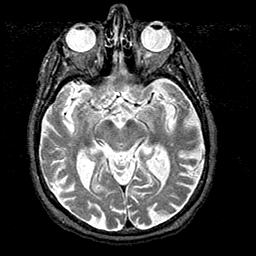
\includegraphics[height = 2.5cm]{Img/S020_MRI.png}}
      \centerline{(a) MRI Image}\medskip
    \end{minipage}
    \hfill
    \begin{minipage}[b]{0.48\linewidth}
      \centering
      \centerline{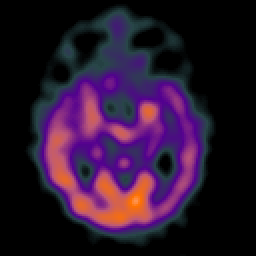
\includegraphics[height = 2.5cm]{Img/S020_SPECT.png}}
      \centerline{(b) SPECT Image}\medskip
    \end{minipage}
    
    \begin{minipage}[b]{0.31\linewidth}
      \centering
      \centerline{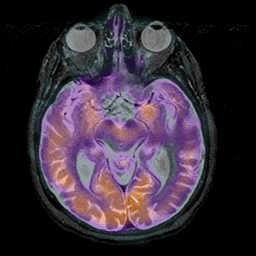
\includegraphics[height = 2.5cm]{Img/S020_Fused_MWT_No_PSO_AVG.png}}
      \centerline{(c) MWT-AVG}\medskip
    \end{minipage}
    \hfill
    \begin{minipage}[b]{0.31\linewidth}
      \centering
      \centerline{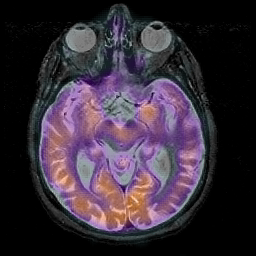
\includegraphics[height = 2.5cm]{Img/S020_Fused_MWT_No_PSO_WANG.png}}
      \centerline{(d) MWT-WANG}\medskip
    \end{minipage}
    \hfill
    \begin{minipage}[b]{0.31\linewidth}
      \centering
      \centerline{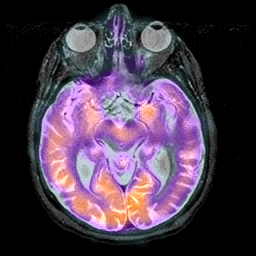
\includegraphics[height = 2.5cm]{Img/S020_Fused_MWT_PSO_Grp.png}}
      \centerline{(e) MWT-PSO}\medskip
    \end{minipage}
    
    \caption{Example of one of the fused images. (a-b) are the MRI and SPECT scans, taken from \cite{HarvardBrain}. Images (c-e) are the fused images obtained using MWT-AVG, MWT-WANG, and MWT-PSO, respectively.}
    \label{fig:ImgFusion}
\end{figure}

\section{Conclusion}
\label{sec:conclusion}
A novel fusion rule using swarm optimization and image fusion performance metric was developed. The obtained results were contrasted with existing fusion rule techniques. It was shown that, regardless of the wavelet transform used, the proposed algorithm increased the mean IFPM value by 0.2 and 0.01 compared to \cite{Wang2004} and average fusion rule for MRI/SPECT image fusion, respectively. Furthermore, the proposed algorithm also displays improved results in terms of other metrics, like entropy and mutual information.
However, the algorithm also had a higher variance in the IFPM and MI metric, which impacts the confidence level for each individual fused image.
Further research should be conducted to bound the variance, and thus improve the confidence and reliability of the fusion results for any medical image pair.
% -----------------------b--------------------------------------------------
\bibliographystyle{IEEEbib}
\bibliography{strings,refs}

\end{document}
